
\documentclass[letterpaper, 10 pt, conference]{ieeeconf}  % Comment this line out if you need a4paper

%\documentclass[a4paper, 10pt, conference]{ieeeconf}      % Use this line for a4 paper

\IEEEoverridecommandlockouts

\overrideIEEEmargins                                      % Needed to meet printer requirements.

%In case you encounter the following error:
%Error 1010 The PDF file may be corrupt (unable to open PDF file) OR
%Error 1000 An error occurred while parsing a contents stream. Unable to analyze the PDF file.
%This is a known problem with pdfLaTeX conversion filter. The file cannot be opened with acrobat reader
%Please use one of the alternatives below to circumvent this error by uncommenting one or the other
%\pdfobjcompresslevel=0
%\pdfminorversion=4

% The following packages can be found on http:\\www.ctan.org
%\usepackage{natbib}
\usepackage{graphicx} % for pdf, bitmapped graphics files
\graphicspath{ {images/} }
%\usepackage{epsfig} % for postscript graphics files
\usepackage{mathptmx} % assumes new font selection scheme installed
\usepackage{times} % assumes new font selection scheme installed
\usepackage{amsmath} % assumes amsmath package installed
\usepackage{amssymb}  % assumes amsmath package installed
\usepackage[mathscr]{euscript}

\title{\LARGE \bf
Power Minimal Optimal Control for Quadrotor UAVs in SE(3)
}


\author{Alexander B. Faustino, TBD, and Timothy Bretl% <-this % stops a space
	\thanks{The authors are with the Department of Aerospace Engineering, Coordinated Science Laboratory, 
		University of Illinois at Urbana-Champaign, Champaign, IL 61801, USA
		\tt\small \{afausti2, tbretl\}@illinois.edu}%
}


\begin{document}

\maketitle
\thispagestyle{empty}
\pagestyle{empty}


%%%%%%%%%%%%%%%%%%%%%%%%%%%%%%%%%%%%%%%%%%%%%%%%%%%%%%%%%%%%%%%%%%%%%%%%%%%%%%%%


\begin{abstract}
	A problem that continues to persist for quadrotor UAVs is their low endurance relative to other prominent UAV platforms. There exist three main approaches to solving this problem: improving hardware efficiency, designing new hybrid systems, and developing software solutions that focus on optimal planning and control. Of the three, software solutions have received the least attention. Existing methods are either heavily constrained, challenging to implement on physical systems, or require significant off-line computation. In this paper we present a method for finding power minimal, smooth trajectories for a quadrotor in SE(3) using exiting models for power and energy consumption. We show that the problem can be formulated as a constrained, continuous time optimal control problem with a polynomial cost function that can be solved numerically. Through simulation we show that our approach, when compared to existing methods, reduces total energy consumption by \textbf{INSERT RESULTS HERE}\% on average. 
\end{abstract}

\section{INTRODUCTION}
\label{intro}
 
The last decade has seen quadrotor helicopters explode in popularity. From an emerging unmanned aerial vehicle (UAV) concept to a prominent research and commercial platform \cite{kumar2012opportunities,hoffmann2007quadrotor} quadrotors have become the nearly ubiquitous aerial robot. Their relative low cost and the simplicity of their dynamics when near hover \cite{bouabdallah2004pid} has made them popular in numerous applications \cite{heng2015efficient,roberts2017submodular,frazzoli2002real}.

The condition of operating near hover also introduces the quadrotor platform's greatest weakness, power efficiency. The power required to keep a quadrotor at hover is approximately 200 W per kg \cite{kumar2012opportunities}. Since quadrotors are rarely flown dynamically far away from hover when used in application, the problem of power efficiency creates a practical limit on their utility. This limit restricts the size of an area that can be explored, the number of images that can be captured by a camera, the mass of potential payloads, etc.. In robotics, maximizing endurance is mostly thought of as a design problem handled by manufacturers. In this paper we present evidence that choices about trajectory and velocity also have a meaningful effect on flight time.

Determining an aerial vehicle's endurance is a common problem in flight mechanics. Solutions for fixed wing and rotor aircraft maximum endurance in steady, forward flight are well known and widely used \cite{anderson2005introduction,leishman2006principles}. Maximum endurance is achieved by traveling at the relative velocity, $V_\infty$, where the power required, $P_{req}$, to overcome the drag force, $D$, is at a minimum. We call this velocity $V_{me}$. 


\begin{figure}[ht]
    \label{QuadDiagram}
	\centering
	
\includegraphics[width=8cm]{placeholder-image.jpg}
	\caption{Coordinate system and flow diagram illustrating induced velocity, force balance at equilibrium, etc..}
\end{figure}


\section{Related Work}
\label{related}

\subsection{Existing white box models}
White box models for quadrotor power consumption are derived from theoretical models for general rotorcraft, mainly presented by Leishman \cite{leishman2006principles}. Leishman's full model has aerodynamic power required for a steady maneuver equivalent to the sum of induced power, parasitic power, profile power, and power required to climb. Aerodynamic power is then scaled by an efficiency factor to convert to electrical power consumed. The individual power terms can be approximated, simplified, or assumed negligible to reduce model complexity. Which of these terms is included and how they are simplified is the main difference between the existing white box models implemented specifically for quadrotors. 

A nearly comprehensive model for power consumption is given by Liu et al. \cite{liu2017power}. Their model contains three of the four terms from Leishman's model relevant to quadrotors: induced, profile, and parasitic, while neglecting the power required to climb. Somewhat similar to the black box models, their model requires initially collecting flight data to numerically determine seven constants. Their model is validated by flying a known trajectory and comparing the estimate of power to the actual power measured onboard. Our experiments are a natural extension to this validation, as we fly similar trajectories with more parameter variation. What differs is that we analyze how the individual terms contribute to the estimate's accuracy rather than just determining the accuracy.

In \cite{bangura2012nonlinear} Bangura and Mahony present a model for mechanical power produced by the rotors as the integral part of their nonlinear dynamic model. They draw on the previous work by \cite{leishman2006principles} and \cite{hoffmann2007quadrotor} to derive a model that more accurately depicts the relationship between the rotors' mechanical and aerodynamic characteristics and the dynamics of the whole body during aggressive maneuvers. While this model has seen success in implementation, the traditional thrust-and-torque-based nonlinear model is still the most prevalently implemented.

\subsection{Trajectory optimization}
Ware and Roy \cite{ware2016analysis} incorporate urban wind data to find more efficient trajectories between two points in the urban canopy layer. Using the wind's prevailing speed and direction above the surrounding buildings as the input to a CFD solver, they generate a grid with 1 m resolution. Similar to \cite{di2015energy} they create a graph for a fixed altitude such that each interior node has eight edges. Using the wind vector, $v_w$, from the CFD solution, they can then choose an upper and lower bounded ground velocity, $v_g$, for the quadrotor such that it minimizes:
\begin{align*}
E_i = \frac{T(v_i + v_\infty \sin{\alpha}) (v_g - v_w) \|d\|}{v_g}
\end{align*}
where $\|d\|$ is the Euclidean distance between the two nodes. They address the acceleration problem encountered by \cite{di2015energy} by constraining the change in velocity, $\Delta v_g$, between edges. Their simulation results show that wind aware planning uses less power than wind naive planning and highlights the importance of having an estimate of the local wind field. We see in the expression for energy consumption that they are only using the dragless model or $P_{ind}$ to minimize power along an edge. We show in Section \ref{sec:Results} that including more terms in their power model, specifically a term for parasitic power, could improve their results.








\section{Quadrotor and Power Model}
\label{model}

In this section we derive our version of the standard quadrotor dynamic model given in \cite{hoffmann2004stanford} and \cite{pounds2002design} specific to the assumptions of level flight and $x^W \times y^W$ planar wind. 

\begin{figure}[t]
    \label{fig:QuadDiagram}
	\centering
	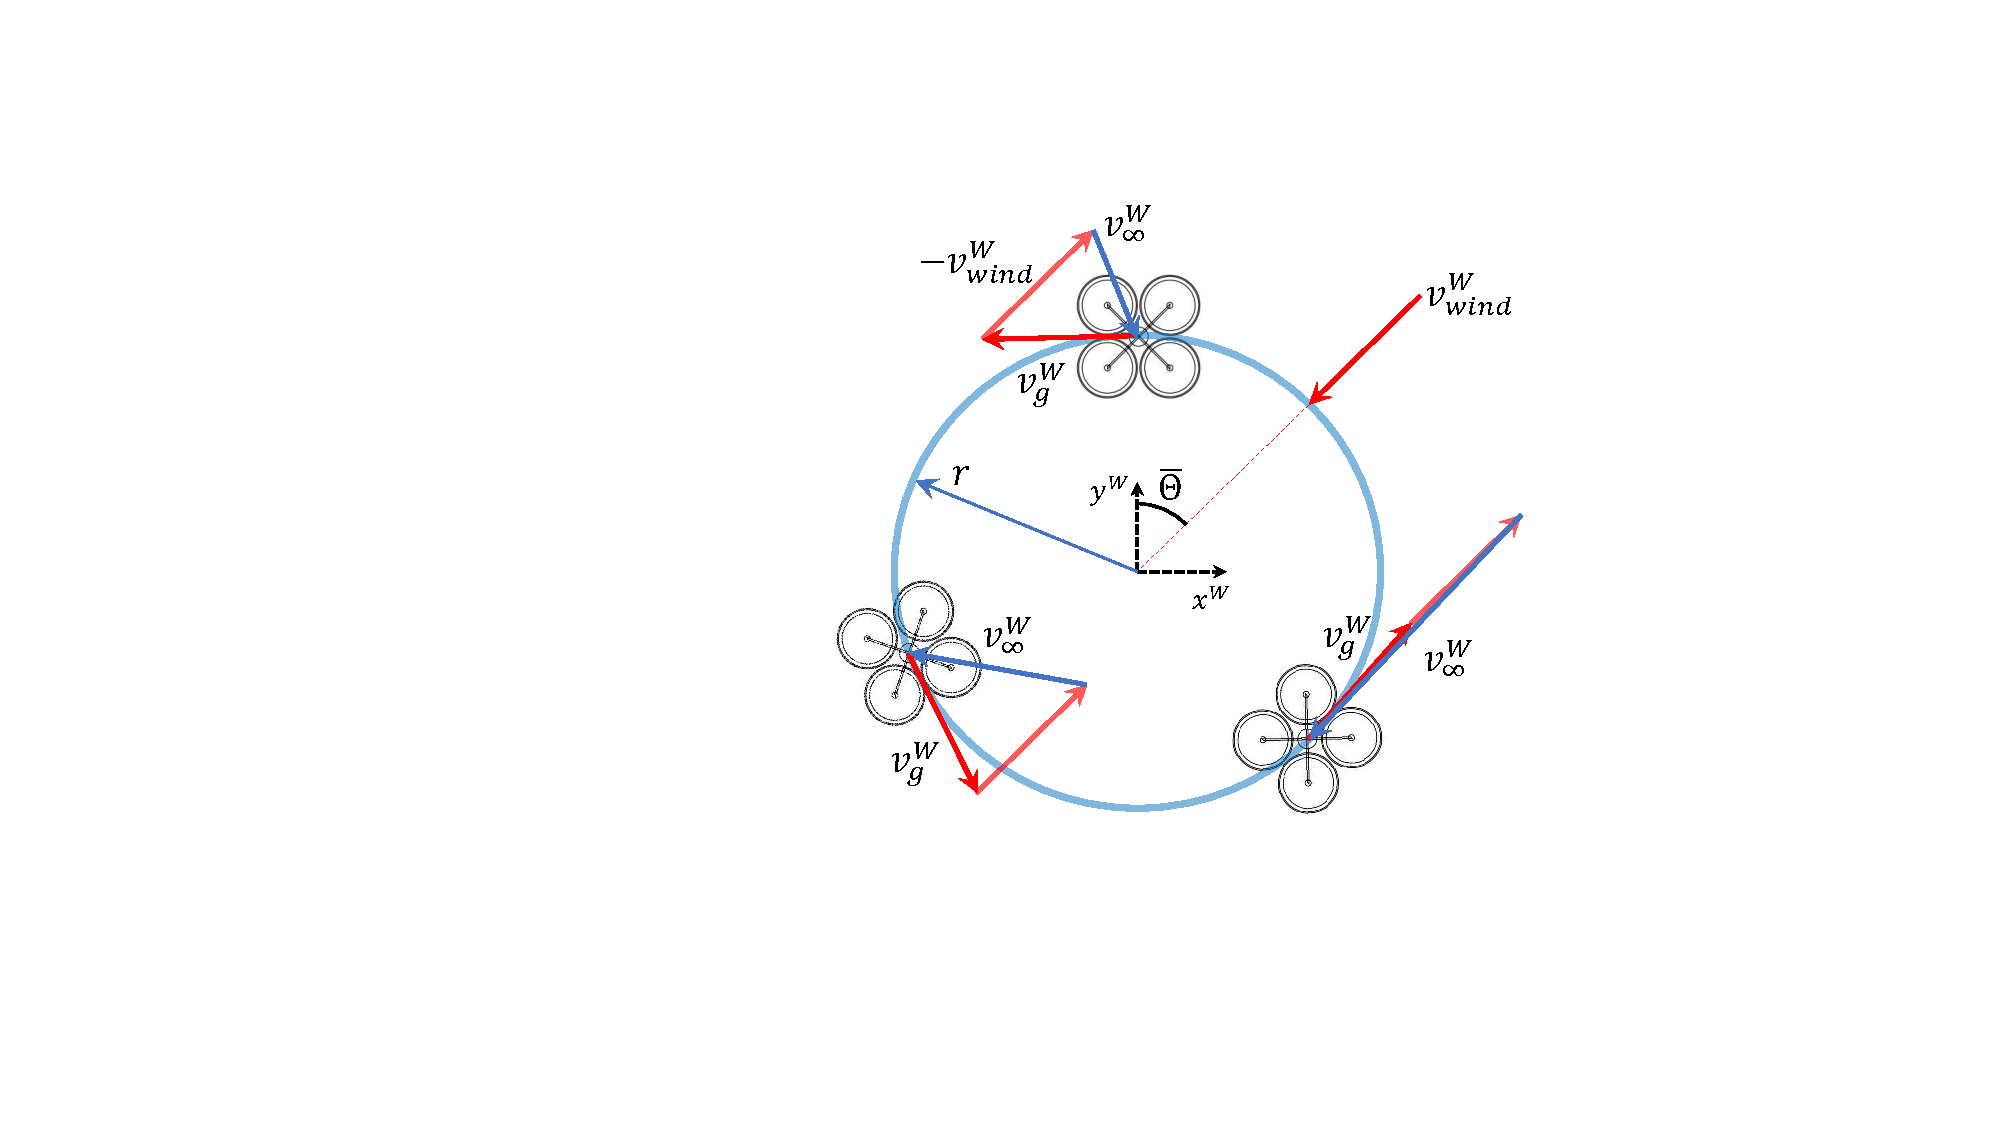
\includegraphics[width=0.5\textwidth, trim={14cm 5cm 8cm 2.5cm},clip]{coordinateDiagram.pdf}
	\caption{Definition of the coordinates used in our analysis. Frame $W$ is defined as a NEU world frame. Frame $B$ (not shown) is attached to the quadrotor's center of mass. Keeping with convention, $z^B$ points down and $x^B$ points forward so that positive pitch angles, $\theta$, correspond to pitching up. We define $\alpha$ as the angle between $\mathbf{v}_\infty^W$ and the rotor plane and $\mathbf{f}_D^W$ so that its direction is always equivalent to $v_\infty^W$. We define the radial position in the orbit by finding the mean wind heading for each experiment, $\bar{\Theta}$, and taking that as 0 radians. We can also see that $\mathbf{v}_\infty^W$ and $\alpha$ vary as the quadrotor moves around the orbit.}
\end{figure}

\subsection{Quadrotor dynamics}
We define two frames of reference, the NEU world frame, $W$, and the body fixed frame, $B$, attached to the quadrotor's center of mass. We also define $R$, a rotation matrix that describes the orientation of $B$ in $W$; $q^{w}=\left(x^W \text{, } y^W \text{, } z^W\right)$, a vector that gives the Cartesian position of $B$ in $W$; and $\mathbf{\omega}^B$, a vector that describes the angular velocity of $B$ with respect to $W$ in the body frame. We parameterize $R$ by the XYZ Euler angle sequence $\Theta=\left(\phi \text{, } \theta \text{, } \psi\right)$ corresponding to roll, pitch, and yaw respectively.

Assuming all four rotors are identical and neglecting blade flapping, each rotor will produce a thrust, $f_j^B \propto \sigma_j$, where $\sigma_j$ is the spin rate of the rotor. Additionally, each rotor will produce a torque, $\tau_j^B$, around each axis of $B$. Torques about $x^B$ and $y^B$ are moments proportional to $\sigma_j$, whereas torques about $z^B$ are pure torques proportional to the difference in spin rate between a rotor and its counter-rotor (i.e. $\sigma_2 - \sigma_4$ and $\sigma_1 - \sigma_3$).

We can then describe the translational and rotational dynamics of the quadrotor as a set of Newton-Euler equations
\begin{align}
    \label{NewtonEqn}
    m \ddot{\mathbf{q}}^W &= R \sum{\mathbf{f}_j^B} + \mathbf{f}_D^W - m\mathbf{g}^W \\
    \label{EulerEqn}
    I^B \dot{\mathbf{\omega}}^B &= -\mathbf{\omega} \times I^B \mathbf{\omega}^B + \sum{\mathbf{\tau}_j}^B
\end{align}
Where $I^B$ is the rotational inertia matrix, which is diagonal when the quadrotor is axisymmetric, the gravity vector is $\mathbf{g}^W=\left(0 \text{, } 0 \text{, } 9.8066\right) \text{ ms}^{-2}$, and $m$ is the mass of the quadrotor in kilograms.

\subsection{Assumption of level flight and planar wind}
By assuming level flight and that $v_{wind}$ is always on the $x^W \times y^W$ plane, we can make two simplifications to reduce our power model's number of parameters. First, rather than having to determine the angle of attack, $\alpha$, we can approximate its cosine and sine with \eqref{cosaoa} and \eqref{sinaoa}.
\begin{align}
	\label{cosaoa}
	\cos \alpha &= \cos \phi \cos \theta \\
	\label{sinaoa}
	\sin \alpha &= \sin \phi \sin \theta
\end{align}
Second, using \eqref{cosaoa} we can approximate the total thrust output by all four rotors, $T$, with just the roll and pitch angles.
\begin{align}
\label{totT}
T &= \frac{mg}{\cos \phi \cos \theta}
\end{align}
This means that our model requires no information about rotor spin rates to predict power consumption.

\subsection{Drag model}
Differing from \cite{tagliabue2019model} and \cite{schulz2015high}, we approximate our drag force with a function cubic in $v_\infty$ rather than quadratic. We did this to avoid overestimating the drag force at lower $v_\infty$ as shown in Fig. 3. We find that a cubic drag model reduces the error in $\hat{P}$ by 28\% on average across all our experiments.
\begin{align}
    \label{DragEqn}
    \mathbf{f}_D^W = \left(\mu_1 v_\infty + \mu_2 v_\infty^2 + \mu_3 v_\infty^3 \right)\frac{\mathbf{v}_\infty}{v_\infty} 
\end{align}
Where $\mu_1$, $\mu_2$, and $\mu_3$ are experimentally determined drag coefficients selected to make \eqref{DragEqn} approximate a more complex drag model such as the ones presented in \cite{huang2009aerodynamics}, \cite{bangura2012nonlinear}, or \cite{leishman2014quadrotors}. We assume that $\mathbf{f}_D^W$ is always co-linear with $\mathbf{v}_\infty^W$ and acts at the quadrotor's center of mass, producing no moments.

\begin{figure}[htbp]
	\centering
	\label{fig:DragModelRegression}
	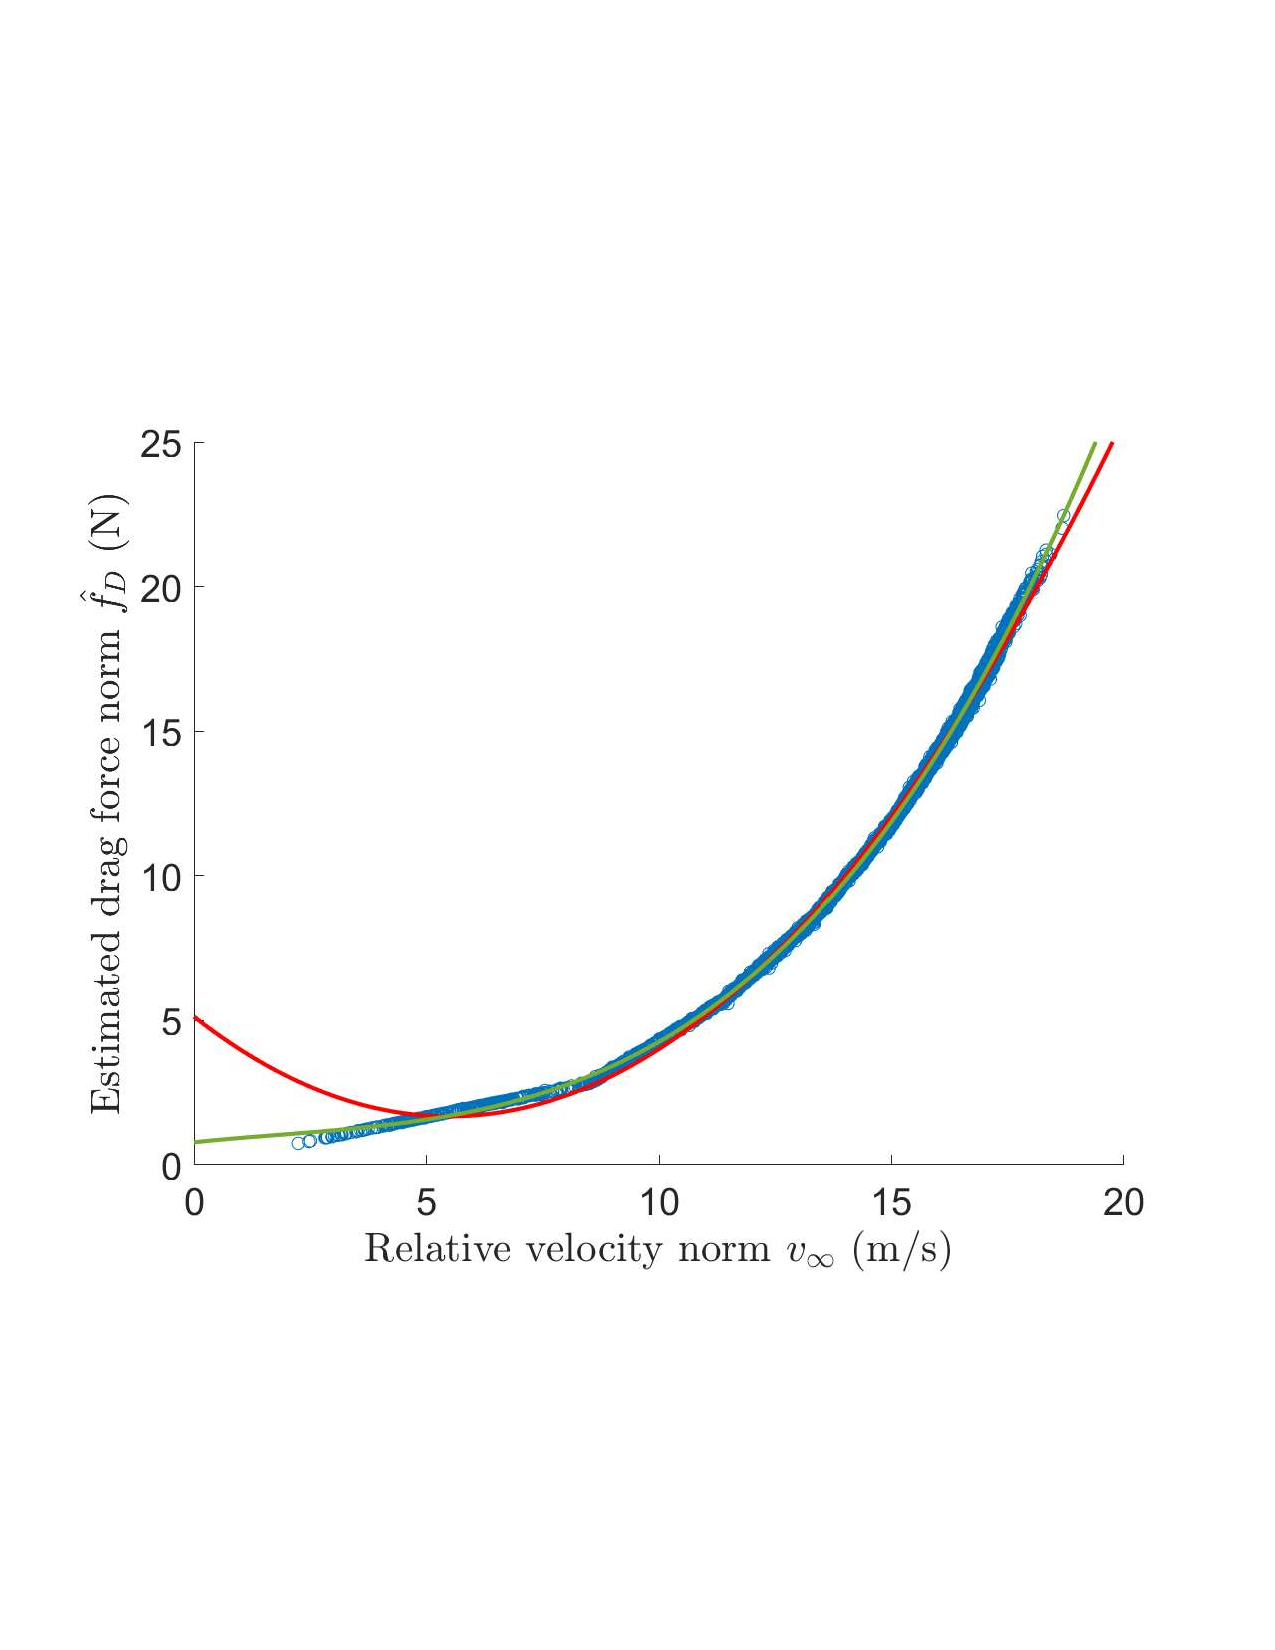
\includegraphics[width=0.5\textwidth, trim={1.25cm 6cm 1.5cm 6cm},clip]{dragModelRegressionWithQuad.pdf}
	\caption{Here we see that the quadratic fit (red) overestimates drag at lower $v_\infty$, whereas the cubic fit (green) closely matches the regression data for the whole range of $v_\infty$. The regression data was collected on level flights not in our experimental set; corresponding drag estimates are based on the residual dynamics of the quadrotor, where we assume thrust and acceleration are known. Drag coefficients for our vehicle: $\mu_1 = 0.1816 \textrm{, } \mu_2 = -0.02326 \textrm{, and } \mu_3 = 0.004045$.}
\end{figure}

\begin{figure*}[h]
	\centering
	\label{fig:relErrMeanGrad}
	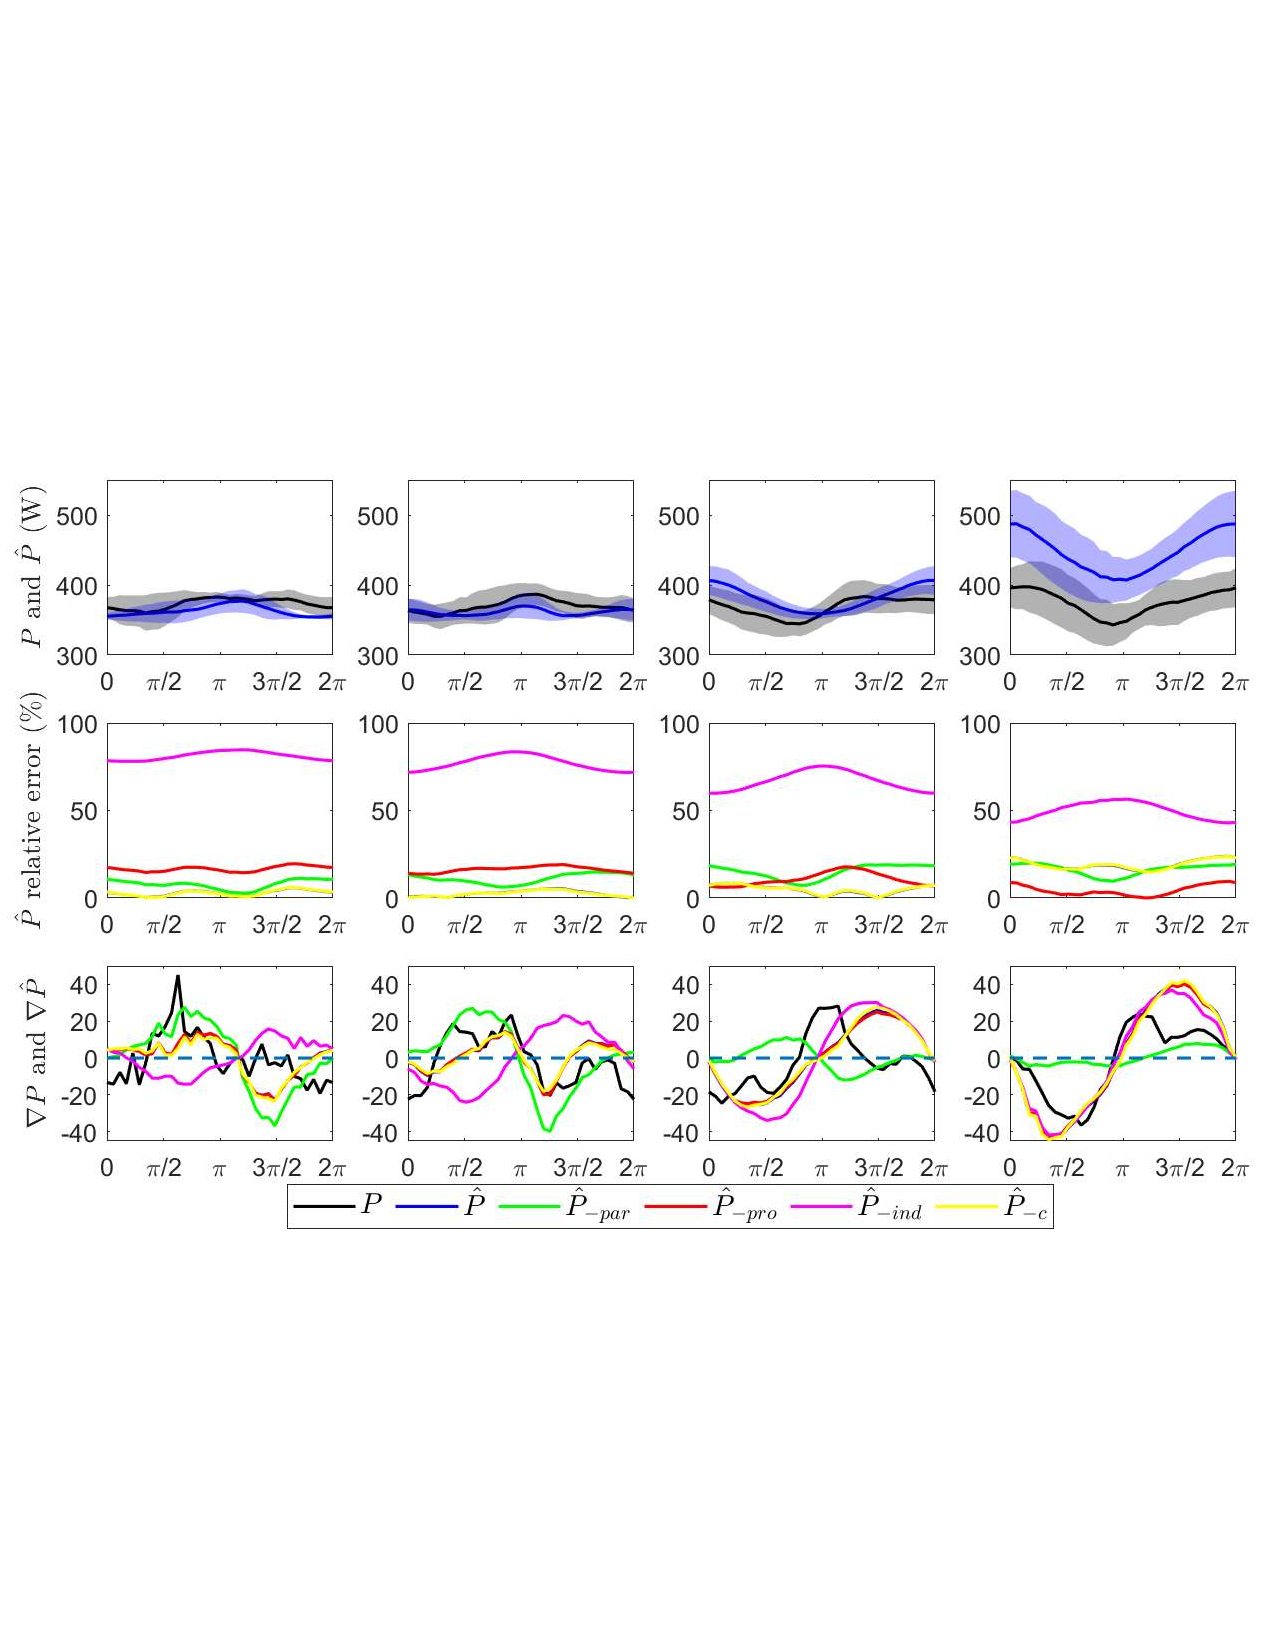
\includegraphics[width=\textwidth, trim={0cm 7cm 0cm 7cm}, clip]{meanCompareAll.pdf}
	\caption{Results for all non-hover flights separated by target $v_g$. Each plot is averaged over all altitudes and orbit radii flown. The x-axis is the quadrotor's position in the orbit in radians, descibed in Fig. 2. From left to right $v_g$ is 2 m/s, 4 m/s, 6 m/s, and 8 m/s. The subscript of $\hat{P}$ denotes which term is removed from the model. \textbf{Top}: Mean $P$ and $\hat{P}$ $\pm 1$ standard deviation. As $v_g$ increases so does the variance of $\hat{P}$. When $v_g$ is 8 m/s we also see a large increase in error, but as seen in the plot directly below, this error can be reduced by neglecting $P_{pro}$. \textbf{Middle}: Relative error between model estimates and measured $P$. We see there is little difference between the full model and the model with $P_c$ removed. Because all our flights were targeting a fixed altitude this is expected. It is also easy to see that the removal of $P_{ind}$ causes the largest error magnitude over all $v_g$. At 8 m/s we see that the inclusion of $P_{pro}$ degrades the accuracy of $\hat{P}$. \textbf{Bottom}: Gradient of $P$ and $\hat{P}$ with respect to position in the orbit. At lower $v_g$ we see that the exclusion of $P_{ind}$ causes the descent direction of the gradient to not lead towards minima in $P$. Although, as $v_g$ increases this problem dissipates. There is a larger amount of error when $P_{par}$ is removed, but in methods using gradient descent magnitude of the gradient is less important than the descent direction being correct.}
\end{figure*}

\subsection{Wind estimation}
The question of how to estimate a wind field onboard a quadrotor has been studied in great detail over the last decade, and continues to be a pressing question in aerial robotics \cite{waslander2009wind, huang2009aerodynamics, gonzalez2019sensing, xiang2016wind}. As seen in Section \ref{sec:Power}, our model is dependent on the output of these models to calculate the freestream velocity's norm, $v_\infty$. For these experiments, we use the output from DJI's built-in method for estimating wind velocity and heading. The accuracy of our model is directly dependent on the accuracy of DJI's model across varied flight regimes. 


\section{Optimal Control Problem}
\label{formulation}

\textbf{COMING SOON}

% linearize around constant velocity
% minimize $P_req$ with $\dot{q}^W$ as decision variable  with fixed initial state, fixed final state and, free final time
% check for feasibility of trajectory

\section{Results and Discussion}
\label{results}

\begin{figure}[ht]
	
\includegraphics[width=8cm]{placeholder-image.jpg}
	\caption{Simulation results.}
\end{figure}

\subsection{Simulation setup}


\section{Conclusions and Future Work}
\label{conclusion}

The results of our experiments are evaluated by assuming two primary use cases for a power consumption model in autonomous UAV planning and control. The first case is predicting the total power consumed by a trajectory, which requires the power consumption model to be accurate across all states in the trajectory. The second case is determining the parameters of minimal power trajectories, where the model’s gradient should have the same sign as the actual power consumed gradient with respect to controllable states. For both cases, our results indicate that a hybrid model based on $v_\infty$ may be necessary.

\subsection{Estimating total power}
As seen in Fig. 4 and Table 1, $P_{ind}$ is by far the largest contributor to accurate estimates of power consumption, especially at lower $v_g$. As expected, the contribution of $P_{par}$ increases with $v_g$, but is still dominated by $P_{ind}$. Interestingly, it is evident that the inclusion of $P_{pro}$ degrades the estimate at greater $v_g$. This could be attributed to the assumption used to neglect a term discussed in \ref{sec:Power} or the method for determining the constant $\kappa_1$. Since all our flights were conducted at near-level flight, it is expected that $P_c$ is nearly negligible.

Table 1 also shows that our full model achieves relative errors lower than previously published models. Since we did not evaluate any of these models using our data, it is not a fair comparison, but it is still worth noting until further verification. This is of particular interest to path and motion planning problems that keep a large margin of battery capacity. By having a better estimate of $P$, uncertainty around max flight time decreases, allowing for a larger feasible trajectory set.

\subsection{Determining minimal power trajectories}
For model-based methods that use gradient descent, it is ideal that the model's computed gradient's descent direction aligns with the descent direction of the underlying physics. Otherwise, the algorithm will converge to non-minimal states. To evaluate this, we approximate the gradient of \eqref{powConsumed} with respect to $v_\infty$, $\theta$, and $\phi$ by taking a finite difference between samples taken while orbiting. In Fig. 4, we see that removing $P_{ind}$ causes discrepancies between the descent directions of $\nabla P$ and $\nabla \hat{P}_{-ind}$. Fig. 4 also shows that this problem diminishes as $v_g$ increases, but as previously stated this magnitude of $v_g$ approaches the current dynamic limit of commercial platforms. Based on that, $P_{ind}$ should always be present in a model where some form of gradient descent is used.

We want to highlight the reliance of our model on accurate estimations of the 3D, time-varying wind field. We think there is room for significant improvement in solutions to this problem, particularly in the atmospheric boundary layer and urban canopies. Looking forward, it will be important to not only estimate the wind vector directly acting on the UAV, like current methods, but to predict the wind field of the entire operating area as well.


%%%%%%%%%%%%%%%%%%%%%%%%%%%%%%%%%%%%%%%%%%%%%%%%%%%%%%%%%%%%%%%%%%%%%%%%%%%%%%%%

%\addtolength{\textheight}{-12cm}   % needs to be before last page to work

%%%%%%%%%%%%%%%%%%%%%%%%%%%%%%%%%%%%%%%%%%%%%%%%%%%%%%%%%%%%%%%%%%%%%%%%%%%%%%%%
%\section*{APPENDIX}

%Appendixes should appear before the acknowledgment.

\section*{ACKNOWLEDGMENT}

Enter shout outs here.

\bibliographystyle{IEEEtran}
\bibliography{sections/references}

\end{document}
